
	\section{ACM/ICPC World Finals 2007}
		\subsection{ACM/ICPC World Finals 2007 A Consanguine Calculations}
			\subsubsection{题目大意}
			ABO 血型由 $i, I^A, I^B$ 三个等位基因确定。$I^A, I^B, i$ 分别产生 A, B, O 型。$I^A, I^B$ 是显性的,而且是共显性的; $i$ 是隐性的。具体地,等位基因型与 ABO 血型的对应情况见表 \ref{ta1}。
				\begin{table}[!htb]
					\centering
					\begin{tabular}{cccc}
						\toprule
							\multicolumn{2}{c}{等位基因}& & ABO 血型   \\
						\midrule
							$ii$&(OO) && O\\
							$I^Ai$&(AO) && A\\
							$I^AI^A$&(AA) && A\\
							$I^Bi$&(BO) && B\\
							$I^BI^B$&(BB) && B\\
							$I^AI^B$&(AB) && AB\\
						\bottomrule
					\end{tabular}
					\caption{等位基因型- ABO 血型}\label{ta1}
				\end{table}
			
			除了 ABO 血型外,还有 Rh 血型。 Rh 血型根据被测者是否具有 Rh 抗原而划分为阴性和阳性。Rh 抗原繁多,故 Rh 血型系统较为复杂,但 只要被测者控制 Rh 等位基因都为隐性(阴性,-),那么被测者的 Rh 血型就是阴性;否则被测者 Rh 呈阳性。 % 所有基因都是显性的。
				
			给定父母子三人中两人的 ABO 血型 和 Rh 血型,判断第三个人可能的 ABO 血型 和 Rh 血型。
			
		\subsubsection{算法讨论}
			枚举父母的 ABO 等位基因和 Rh 等位基因,判断是否满足给定条件,再根据孟德尔定律判断孩子的等位基因,导出孩子的血型。
			
			取出所有满足条件的情况,去重后作为答案输出。
			
			\subsubsection{时空复杂度}
				时间复杂度 $\mathcal{O}\left(1\right)$。内含常数 $(6 \times 4)^2 \times 2 \times 2 = \num{2304}$。
					
				空间复杂度 $\mathcal{O}\left(1\right)$。
		\newpage

	
		\subsection{ACM/ICPC World Finals 2007 E Collecting Luggage}
			\subsubsection{题目大意}
			如图 \ref{2007e},机场的行李提取轨道为一简单多边形。给定
			行李的起始位置,速度,以及人的起始位置,速度。不跨越轨道,求人拿到行李的最短时间。人的速度快于行李速度。
				\begin{figure}[htb]
					\centering
					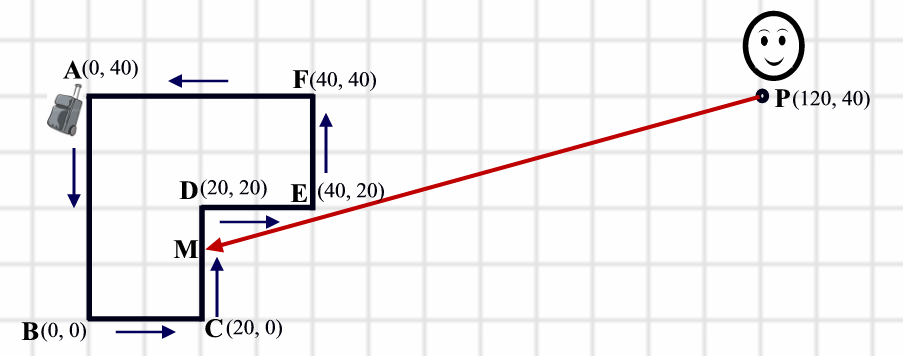
\includegraphics[width=0.7 \textwidth]{2007e.png}
					\caption{行李提取轨道} \label{2007e}
				\end{figure}
			
			行李轨道的顶点数 $N \le 100 $。
		\subsubsection{算法讨论}	
			由于人的速度快于行李速度,故提取到了行李后,也可以磨蹭时间,跟着行李同步走,于是乎答案单调。可以先二分,将问题简化成判定性问题。
			
			设二分的时间 $t_0$,那么需回答 $t = t_0$ 时刻,人能否拿到行李。行李的轨迹是固定的,可以算出其在 $t = t_0$ 时的位置。那么只需确定人能否在  $t = t_0$  时刻赶到行李处;或者说,求出到达该行李处的最短时间,看其是否不超过 $t_0$。
			
			要最快地到达行李在 $t = t_0$ 的位置,可以证明只需在起点,终点,多边形顶点间走直线。此命题较经典,故在此节省篇幅省去证明。枚举两点,判断是否跨越多边形,如果没有跨越,就加边,直到完成建图。最后只需运行 Dijkstra 等最短路算法即可求出最短时间,与 $t_0$ 比较,反馈给二分搜索。
			
			\emph{一些最短路的询问可以预先处理,因为二分算法询问的时间 $t_0$ 不会修改这些信息。}
			
			最终的答案由二分搜索给出。
					
			\subsubsection{时空复杂度}
				由于预处理,时间复杂度 $\mathcal{O}\left(k + N^2\right)$。$k$ 是二分的次数,与精度有关。
					
				空间复杂度 $\mathcal{O}\left(N^2\right)$。
		\newpage
					
	
		\subsection{ACM/ICPC World Finals 2007 F Marble Game}
			\subsubsection{题目大意}
			如图 \ref{2007f},一个 $N \times N$ 的板子上有 $M$ 个球 $M$ 个洞,且一一对应。倾斜板子(上下左右)可使得球滚动。\emph{必须等到球滚动停止,才能更改倾斜方向。球入洞后,会填平空隙。}设计一种方案,倾斜最少的次数,使得球对号入座。
				\begin{figure}[htb]
					\centering
					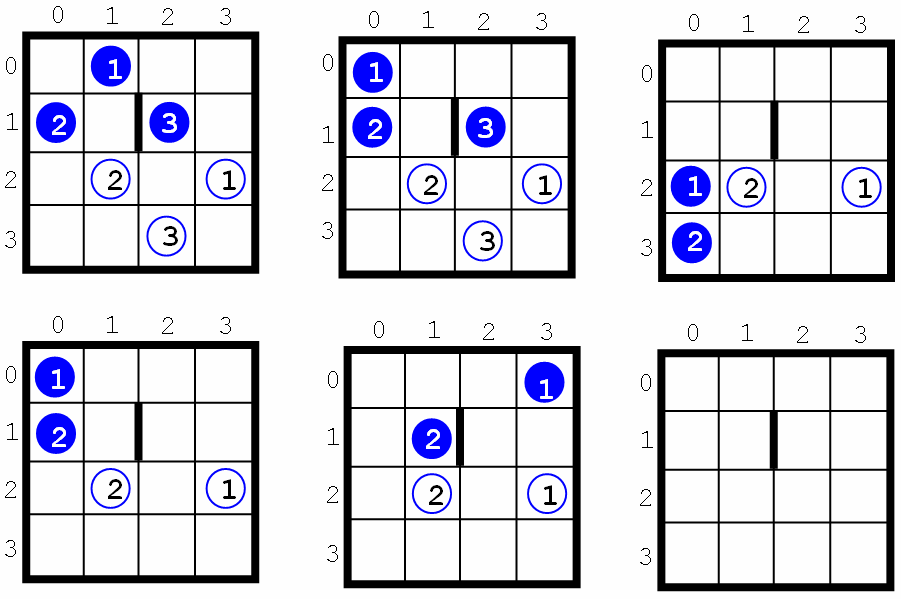
\includegraphics[width=0.7 \textwidth]{2007f.png}
					\caption{} \label{2007f}
				\end{figure}
			
			$N \le 4$。 
			
			\subsubsection{算法讨论}
				直接从起始局面开始 BFS,枚举四个方向,并模拟当前的情况,将搜索出的情况加入队列。
				
				去重可使用 set 等 STL。
				
				情况数的最大值为 $\binom{4 \times 4}{4 \times 4 / 2} = 12870$。
				
			\subsubsection{时空复杂度}
				时间复杂度 $\mathcal{O}\left(N^2f(N) N^2\log f(N)\right)$。 $f(N)$ 表示情况数。题中 $f(N) \le 12870$。
					
				空间复杂度 $\mathcal{O}\left(N^2f(N)\right)$。
				
			
		\newpage
					
	
		\subsection{ACM/ICPC World Finals 2007 H Raising the Roof}
			\subsubsection{题目大意}
				\emph{空间}中有若干三角形,且两两不交(不含边界)。一束平行光从上往下照射,被照到的部分需染色。问总计需染色多大的面积。
				
				三角数 $N \le 1000$,顶点数 $M \le 300$。
			\subsubsection{算法讨论}
				先将空间问题平面化。根据射影定理,如果一个面积为  $S$ 三角形在平面 $\alpha$ 的投影的面积为 $S^\prime$,那么此三角形与平面 $\alpha$ 的二面角 $\theta$ 满足
				\begin{align}
					\cos \theta = \frac{S^\prime}{S} \label{07hhhh}
				\end{align}
				根据 \eqref{07hhhh}, $S = S^\prime / \cos \theta$,故忽略掉高坐标后,相当于一个带权的平面三角面积并,每个三角的权为与 $xOy$ 平面的二面角的倒数  $1/ \cos \theta$。 一个细节是要先删除掉完全竖直的三角形,因为其本身投影到 $xOy$ 平面相当于一条直线,不影响答案,但权值为 $\infty$。
				
				随后考虑这个平面问题。求出所有交点,将纵坐标取出并排序,就可以将整个平面划分为若干横条。可以证明各个横条中要被计算的图形都是梯形(满足线性),故只需对各个横条的中点扫描,乘上横条的粗细,计入答案即可。
				
				注意到我们需要维护处于(空间中)最高点的图形的权值,此处可以用扫描线 + 平衡树。对于横条的中线,每个三角形与其交必然是区间(或者空集),将左端点视为插入,右端点视为删除,以高度来维护三角形集的信息。在相邻事件的中点,需要求到最上的三角形的权值,将其乘上相邻事件的长度,求和并返回即可。
					
			\subsubsection{时空复杂度}
				时间复杂度 $\mathcal{O}\left(N^3\log N\right)$。上限较宽松,程序运行速度还是满意。
					
				空间复杂度 $\mathcal{O}\left(N\right)$。
				
			
			
		\newpage
					
	
		\subsection{ACM/ICPC World Finals 2007 I Water Tanks}
			\subsubsection{题目大意}	
				
				如图 \ref{2007i},有 $N$ 个等粗的水缸,第一个开口,与大气接触,其余的水缸相邻两个间都有一个管道,体积不计,且\emph{高度递增}。问将第一个水缸灌满须多少水。
				
				
				\begin{figure}[htb]
					\centering
					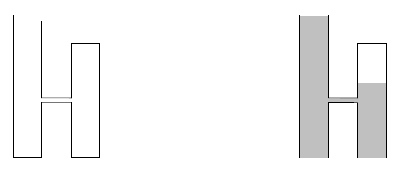
\includegraphics[width=0.7 \textwidth]{2007i.png}
					\caption{水缸灌水前后} \label{2007i}
				\end{figure}	
			
				$N \le 10$。标准大气压 $p_0$,水的密度 $\rho$,重力加速度 $g$%,水缸底面积 $S$,水缸高度 $h_i$ 
				已知
				,玻意耳-马略特定律
				\begin{align}
					p_1 V_1 = p_2 V_2
				\end{align}
			\subsubsection{算法讨论}
				先假设第一个水缸的高度无穷大,%这样
				即我们可以一直灌水。这样整个灌水过程可以描述为
				\begin{enumerate}
					\item 先把第一个水缸灌到管道处,紧接着第二个水缸也被灌到了管道处。
						此时第二个水缸到其后所有水缸的气体封闭。$i = 2$。
					\item 第 $i$ 个水缸因为第一个水缸的水压,致使水面缓缓抬升,气体压缩。如果第一个水缸的液面高度 $h_1$,压缩前 第 $i$ 个水缸到最后一个水缸的气体的压强 $p$,体积 $V$,第 $i$ 个水箱与第 $i - 1$ 个水箱的管道高 $H$
					,这样此水缸的高度 $h_i$ 满足
						\begin{align}
							(\rho g \cdot (h_1 - h_i) + p_0) \cdot (V - S \cdot (h_i - H)) = p V \label{2007i}
						\end{align}
					且从 \eqref{2007i} 中可以看到 $h_1$ 随 $h_i$ 的单调性。如果 $i = n$ ,则此阶段一直进行;否则此阶段直到 $h_i$ 上升到其与 $(i + 1)$ 号水箱间的管道处为止。
					\item $h_i$ 不再变化,水流向 $h_{i+1}$。此时的方程与  \eqref{2007i} 类似:
						\begin{align}
							(\rho g \cdot (h_1 - h_i) + p_0) \cdot (V - S \cdot (h_i - h_{i+1} - H)) = p V \label{2007i2}
						\end{align}
						$h_1$ 随 $h_i$ 单调。此过程直到 $h_{i+1}$ 上升到 $i$ 号水箱与 $(i + 1)$ 号水箱间的管道处为止。
						此时 第 $i$ 个水箱 的气体单独封闭,此部分的气体质量不会再变化。\emph{令 $i$ 自增一},则第 $i$ 个水缸到其后所有水缸的气体再次封闭。跳到步骤 2。
				\end{enumerate}
				
				如果按照此步骤一直进行下去,$h_1$ 将会 $\to + \infty$。而 $h_1$ 只需上升到某一特定值即可退出程序,故某一阶段可能会执行到一半就会中断退出。不过没关系,确定了退出时的 $h_1$ 就可以根据  \eqref{2007i} \eqref{2007i2} 解出对应的 $h_{i, i+1}$,二分或者数学方法皆可。最后用 玻意耳-马略特定律 更新一下单独封闭掉的气体体积,求个和,从水箱总体积里扣去就是答案。
			
			\subsubsection{时空复杂度}
				时间复杂度 $\mathcal{O}\left(N k\right)$。$k$ 是解方程是二分的次数,与精度相关。
					
				空间复杂度 $\mathcal{O}\left(N\right)$。
				
		\newpage
					
	
		\subsection{ACM/ICPC World Finals 2007 J Tunnels}
			\subsubsection{题目大意}
				有向图 $G = (V, E)$。一个人从 $s \in V$ 开始走,$t \in V$ 是终点。你可以随时监控他的位置,并每次在其到达某一节点后,就可以删除某些边。问至少删除多少条边,才能使得其无法到达终点。
				
				$N = |V| \le 50, M = |E| \le 100 $。
			\subsubsection{算法讨论}
				此问题看起来像是最小割问题——将 $s, t$ 割开,使其不连通。但是仔细分析下就会发现这个问题并没有这么简单,因为可以监控其行走的轨迹,故可以在其行动之后,根据其选择再进一步决定删边的方案。
				
				为了解决这一问题,我们对于每个点 $v \in V \setminus \{ t\}$,定义一个变量 $F(v)$,使得其最终将会变成此人从 $v$ 开始走的情况下,保证不到达 $t$ 最少须删除的边数。
				
				初步的算法流程如算法 \ref{2007jalgo}。%下
				\begin{algorithm}[H]
				\caption{求出正确的 $F(x)$}
				\label{2007jalgo}
					\begin{algorithmic}[1]
						\State $F(\cdot) \gets + \infty$
						\For{如果此人在 $u$ 点,删掉 $x$ 条边后,必须经过 $F(v)$ 值 $\le y$ 的点 $v$才能出去}  \label{2007jaaa}
							\If{$F(u) > x + y$}
							\State $F(u) \gets x + y$
							\EndIf
						\EndFor
					\end{algorithmic}
				\end{algorithm}
				\begin{algorithm}[tbh]
				\caption{求出正确的 $F(x)$ ver. 2.0}
				\label{2007jalgo2}
					\begin{algorithmic}[1]
						\For{$u \in V \setminus \{ t\}$}
							\State $F(u) \gets \Call{MinCut}{u, t}$
						\EndFor
						\State 设置所有 $v \in V \setminus \{ t\}$ 为未访问的点
						\For{还剩下未访问的点} 
							\State $Min \gets \min_{\text{未访问过的}\, x}{F(x)}$
%							\If {$Min = +\infty$}
%								\State \textbf{break}
%							\EndIf
							\State 访问所有满足 $F(v) = Min$ 的 $v$,并在图 $G = (V, E)$ 中删除它们 \Comment{$F$ 值已经固定。}
							\For{未访问过的  $x$ } 									 \Comment{更新$(y = Min)$。}
								\If{$F(x) > \Call{MinCut}{x, t} + Min$}
								\State $F(x) \gets \Call{MinCut}{x, t} + Min$
								\EndIf
							\EndFor
						\EndFor
					\end{algorithmic}
				\end{algorithm}
				
				我们稍后将会证明算法 \ref{2007jalgo} 第  \ref{2007jaaa} 行中找 $(u, x, y)$ 的顺序不会影响答案,以及算法 \ref{2007jalgo} 的正确性。
				
				进一步观察,发现 一旦确定了 $u, y$ 的值后,可将所有的  $F(v)$ 值 $\le y$ 的点 $v$ 删去,求最小割,即可求到最小的 $x$ 值。
				而所有的 $f(\cdot)$ 都在不断下降,故只有较小的 $f(\cdot)$ 才能够更新较大的 $f(\cdot)$。不妨从小往大确定 $f(\cdot)$ 的正确值。进一步优化后可得出算法 \ref{2007jalgo2}。此算法能在 $\mathcal{O}\left( N^2MaxFlow(N, M) \right)$ 的时间复杂度内出解。$Maxflow(N, M)$ 是求解 $N$ 个点 $M$ 条边的网络流的时间。
				
				以下是此算法的正确性证明。
				\begin{theorem} \label{2007jaaaaa}
						算法 \ref{2007jalgo} 第  \ref{2007jaaa} 行中找 $(u, x, y)$ 的顺序不会影响答案。
				\end{theorem}
				\begin{pf}
					算法执行过程中,$G = (V, E)$ 不会变化,$F(\cdot)$ 单调下降,故若某一时刻起,  $(u, x, y)$  是算法  \ref{2007jalgo} 第  \ref{2007jaaa} 行要寻找的项(下称“可行优化”),那么他将一直成为可行优化,直到其被处理为止。\qed
				\end{pf}
				\begin{theorem}
						算法 \ref{2007jalgo} 提供的 $F(s)$ 值是足够的。
				\end{theorem}
				\begin{pf}
					如果最后一次更新 $F(s)$ 的操作是 $(s, x, y)$,那么我们可以删掉 $x$ 条边,把它逼到一个 $F(s^\prime) \le y$ 的点 $s^\prime$,然后继续下去,这一步不会超过 $F(s^\prime)$ 次删除(归纳),在加上前面的 $x$ 次删除,故总计 $F(s)$ 次删除足矣。\qed
				\end{pf}
				\begin{lemma}
						设图 $G = (V, E), G^\prime = (V, E \setminus \{e\})$,$G$ 中 $x$ 点的 $F(x)$ 值为 $F_1(x)$,$G^\prime$ 中 $x$ 点的 $F(x)$ 值为 $F_2(x)$,则 $\forall x \in V, F_1(x) - 1 \le F_2(x)  \le F_1(x)$。
						\label{2007jlemma}
				\end{lemma}
				\begin{pf}
					因为 $G$ 比 $G^\prime$ 多一条边,故所有能在 $G$ 中执行的可行优化 $(u, x, y)$ 在 $G^\prime$ 中肯定能实施,故  $\forall x \in V, F_1(x)\ge F_2(x)  $。
					
					根据定理 \ref{2007jaaaaa},可以假设一开始算法将 $G^\prime$ 的 $F(\cdot)$ 值被优化成了跟 $G$ 最终一模一样的情况$(F_1(x) = F_2(x))$。不是一般性,我们可以假设此算法每次都对 $F_2(\cdot)$ 减少 1。
					下说明,接下来同一个点 $u$ 的 $F_2(u)$ 不会被优化两次。
					
					先考虑第一次 $F_2(u)$ 被 $(u, x, y)$ 优化的情况。由于其不适用于 $G$,故有以下可能
						\begin{enumerate} 
							\item 在 $G^\prime$ 中删掉这 $x$ 条边后,有一条到达终点的路径不经过一个 $F_1$ 值 $\le y$ 的点,而其经过了一个 $F_2$ 值 $\le y$ 的点 $v$。此处应假设还暂时没有点的 $F_2$ 值被优化两次,故 $F_2(v)$ 已经被优化过了,$F_2(v) = y$,$G$ 中 $F_1(v) = y + 1$,而需注意 $F_2(u) = x + y \ge x = F_2(v) $。
							\item  在  $G^\prime$ 中删掉这 $x$ 条边后,所有到达终点的路径都会经过一个 $F_1$ 值 $\le y$ 的点,而其不能对 $F_1(u)$ 优化显然是因为 $G$ 中多了一条原先被删除的边 $e$ 后,给了 $u$ 到终点的一条不经过  $F_1$ 值 $\le y$  的点的路径。于是乎, $(u, x + 1, y)$ 才适用于 $F_1(u)$。这样,必然存在一条 $u$ 到 $e$ 的一个端点 $e_0$ 的路径,其不经过任何一个  $F_1$ 值 $\le y$ 的点 。否则的话所有经过  $e$ 到达终点的路径都会经过一个 $F_1$ 值 $\le y$ 的点,致使 $(u, x, y)$ 适用于优化 $F_1(u)$,从而造成矛盾。因此,$(e_0, x + 1, y)$ 也适用于 $F_1(e_0)$,因为删掉这 $x$ 条边和 $e$ 后,就不会有不经过 $F_1$ 值 $\le y$ 的点到达终点的路径,因为如果不是这样,那么可以利用刚才的提到的路径,结合不经过 $F_1$ 值 $\le y$ 的点从 $e_0$ 到达终点的路径,将其延伸成一条不经过 $F_1$ 值 $\le y$ 的点从 $u$ 到终点的路径,与 $(u, x, y)$ 不适用于 $F_1(u)$ 造成矛盾,于是乎,$F_1(e_0) \le x + y + 1 = F_2(u) + 1$。
						\end{enumerate}
						
						综上,可以说明对于任意优化了的  $F_2(u)$, $F_1(e_0) \le F_2(u) + 1$。
						接下来,考虑第二次 $F_2(u)$ 被 $(u, x, y)$ 优化的情况。由于其还是不适用于 $G$,故仍有以下可能
						\begin{enumerate} 
							\item 在 $G^\prime$ 中删掉这 $x$ 条边后,有一条到达终点的路径不经过一个 $F_1$ 值 $\le y$ 的点,而其经过了一个 $F_2$ 值 $\le y$ 的点 $v$。与前面的同理,必然有一个 $F_2(v)$ 从 $y + 1$ 减少到了 $y$。根据前面的判断, $F_1(e_0) \le y + 1$。故  $(u, x, y + 1)$ 是适用于 $F_2(u)$ 的:不使用 $e$ 的必然跨过一个 $F_1$ 值 $\le y + 1$ 的,(因为目前应假设还暂时没有点的 $F_2$ 值被优化两次)也就是 $F_2$ 值 $\le y$,这是满足我们的假设的;而适用 $e$ 的必然经过 $e_0$, $F_1(e_0) \le y + 1$。这样 $F_1(u) = x + y + 1, F_2(u) = x + y$,与其为第二次优化是互相矛盾的。
							\item 在  $G^\prime$ 中删掉这 $x$ 条边后,所有到达终点的路径都会经过一个 $F_1$ 值 $\le y$ 的点。这样  $(u, x + 1, y)$ 是适用于 $F_2(u)$ 的:删掉 $e_0$ 和这 $x$ 条边,变成与 $G^\prime$ 相似的情况。这样 $F_1(u) = x + y + 1, F_2(u) = x + y$,与其为第二次优化是互相矛盾的。
						\end{enumerate}
					
					综上,只能每个 $F_2(x)$ 优化一次并减少 $1$,引理得证。 \qed

				\end{pf}
				
				\begin{theorem}
						算法 \ref{2007jalgo} 提供的 $F(s)$ 值是必要的。
				\end{theorem}
				\begin{pf}
					设我们只有 $F(s) - 1$ 次删边操作,那么此人会寻找一条通往终点,不经过 $F$ 值低于 $F(s)$ 的路径(否则可以进行 $(s, 0, y), y < F(s)$ 的优化,与条件矛盾),直到我们进行了一次删边操作。删边前,此人所在点的 $F$ 值 $ \ge F(s)$,根据引理 \ref{2007jlemma},删边后,此人所在点的 $F$ 值 $ \ge F(s) - 1$,而我们还剩下 $F(s) - 2$ 次删边操作。重复迭代上述操作,当此人所在点的 $F$ 值 $ \ge 1$ 时,我们就不能再删边了,这样它就可以直接走向出口了 
%					{\rm
%					( ̄\hskip-0.05em$\bigtriangledown$\hskip-0.05em ̄ ") 
%					(" ̄$ \bigtriangledown $ ̄)/}
					。
					故 $F(s) - 1$ 次删边是不足的。\qed
				\end{pf}
				至此,本算法的所有正确性说明完毕。
			\subsubsection{时空复杂度}
				时间复杂度 $\mathcal{O}\left( N^2 MaxFlow(N, M)\right)$。$Maxflow(N, M)$ 是求解 $N$ 个点 $M$ 条边的网络流的时间。
					
				空间复杂度 $\mathcal{O}\left(N + M\right)$。
				
		\newpage
					
				